\begin{abstract}
Omnipair Dusk combines exchange, isolated lending, two-sided liquidity shares, and leveraged liquidity vaults in one market on Solana. Its accounting identity separates cash, indexed cash-backed debt, and vault-owned reserve claims. Swap execution applies a second separation: unpaid cash-backed interest is excluded from curve principal, and hLP ownership is removed to obtain the ordinary liquidity tranche on which traders execute. A full-range constant-product tail and two nested liquidity bands define a continuous, piecewise analytic reserve path. After a trade, the program reconstructs hLP ownership and opposite-asset funding algebraically. Credit uses conservative internal price and depth observations, while realized yield, recenter funding, and loss recovery have distinct accounting paths. This paper describes the implemented mechanisms and their limitations, with reproducible numerical illustrations of the curve, interest controller, and hLP recovery incentives.
\end{abstract}

\textbf{Implementation scope.} This revision follows Dusk source at commit
\texttt{263c1635ad87} (September 10, 2026). Dusk is under active development and has not been deployed to production. Equations below suppress token normalization and integer rounding unless stated otherwise. The source map and generated examples accompany both drafts; numerical illustrations are not an audit, market backtest, or return forecast.

\section{Introduction}

An AMM, a lending market, and a liquidation route often hold separate views of the same asset. A lender may value collateral at a linear price even though recovery must occur through a finite pool. For a thinly traded pair, the difference between that mark and executable recovery can dominate the economics of the loan. External price feeds can improve information, but do not create the inventory required to liquidate a position.

Dusk develops Omnipair's Generalized Automated Market Maker (GAMM) approach: exchange and credit share a pair-local balance sheet \cite{omnipair-docs-gamm}. Borrowing replaces available cash with a debt claim, while trading changes the inventory coordinate. The market also maintains two aggregate hLP vaults, each targeting exposure to one asset through a funded position in the market's own liquidity shares. The intended benefit is a common accounting and settlement system for activities that otherwise depend on separate venues.

The current design has three important separations. First, stored reserve claims differ from cash available for a transfer. Second, the coordinate used to mint and burn liquidity shares differs from the ordinary tranche used to quote a swap. Third, collateral admission, liquidation eligibility, and actual liquidation proceeds use different valuations. These distinctions are necessary once an AMM contains debt, concentrated liquidity, and leveraged ownership at the same time.

``Oracle-less'' means that the program does not require an external price feed to execute these mechanisms. It does use internal price observations, moving averages, depth measurements, and a persistent concentration center. Their quality depends on the market's trading history. Market-local accounting contains a loss within its accounting domain; it does not establish an external fair price or guarantee that liquidity remains available.

\ifexpanded\else
The design sits within a broader AMM lineage: Curve's StableSwap and dynamic-peg work explored concentrating liquidity and adapting an internal price reference \cite{curve-stableswap,curve-cryptopools}. Egorov's leveraged-liquidity analysis and Yield Basis motivate the one-sided LP exposure problem \cite{egorov-yieldbasis-whitepaper,yieldbasis-technical}. Dusk's particular contribution is the integration of curve execution, ownership, and funding within one market; this paper makes no comparative performance claim.
\fi

\ifexpanded
\subsection{Related mechanisms}

StableSwap demonstrated how an invariant can allocate more liquidity near an expected exchange rate \cite{curve-stableswap}. CryptoSwap developed internal price adaptation and an economic budget for moving concentrated liquidity \cite{curve-cryptopools}. Dusk uses a different curve construction: a nonzero constant-product tail plus nested core and shoulder ranges, with an explicit custody bucket for retained recenter funding. The mathematical form and financing of that movement must therefore be evaluated on their own terms.

The adaptive rate-at-target idea is closely related to Morpho's AdaptiveCurveIRM \cite{morpho-irm-github}. Dusk implements its own bounded, discrete anchor update and accrues a shared asset-side borrow index. Similar controller intuition does not imply identical integration, parameters, or numerical behavior.

Leveraged liquidity has a separate lineage. Egorov's treatment of constant-product LP convexity motivates one-sided exposure through dynamically maintained leverage \cite{egorov-yieldbasis-whitepaper}. Yield Basis holds Curve LP collateral against crvUSD debt; its LEVAMM and VirtualPool support the rebalance mechanism \cite{yieldbasis-technical}. Dusk represents the LP ownership and funding inside the same market and reconstructs them at the quoted endpoint. Section~\ref{sec:hlp} makes the scope of that distinction precise.

\subsection{What is established here}

The reserve identities and endpoint formulas are accounting statements. Their continuous forms can be derived and checked independently. Whether the Rust program preserves them under every token decimal configuration, overflow boundary, account combination, and instruction sequence is an implementation question. Whether a configured market offers useful credit and sustainable LP returns is an empirical question. The examples at the end address selected arithmetic properties, while the expanded appendices connect those properties to source and describe the remaining evaluation work.
\fi

\section{Market Accounting}

Consider base and quote assets, denoted $b$ and $q$. For each side $i$, write $C_i$ for accounted reserve cash, $D_i^f$ for indexed public-borrow debt, $D_i^\ell$ for indexed isolated-leverage debt, and $H_i$ for the aggregate hLP live-reserve component. The stored live reserve is
\begin{equation}
\boxed{R_i=C_i+D_i^f+D_i^\ell+H_i.}
\label{eq:ledger}
\end{equation}
Here $D_i^{\rm cb}=D_i^f+D_i^\ell$ is all cash-backed debt. Isolated leverage is a separate health domain, but is already included in cash-backed debt. hLP funding debt $D_i^h$ affects utilization and vault equity; it is not added again to the cash-backed term.

Let $P_i^f$ and $P_i^\ell$ be the outstanding principal counters. Unpaid cash-backed interest is
\begin{equation}
J_i=\pos{D_i^f-P_i^f}+\pos{D_i^\ell-P_i^\ell}.
\end{equation}
The executable reserve coordinate before separating hLP ownership is
\begin{equation}
X_i=R_i-J_i.
\label{eq:principal}
\end{equation}
Thus interest accrual can increase the stored live reserve without expanding the curve principal. Using $R_q/R_b$ as a universal swap price would miss both this adjustment and concentrated-curve geometry.

\subsection{Cash, custody, and liquidity shares}

Accounted cash is only one claim on the physical reserve vault. Claimable swap fees, hLP backing inventory, and protected recenter reserves also occupy custody. The program requires physical tokens to cover their sum:
\begin{equation}
V_i^{\rm reserve}\ \ge\ C_i+F_i^{\rm custody}+B_i^b+B_i^q+Z_i,
\label{eq:custody}
\end{equation}
where $B_i^b,B_i^q$ are backing inventory assigned to the two hLP vaults and $Z_i$ is protected recenter funding. An unsolicited token donation does not automatically increase executable liquidity. Interest-vault accounting is separate from this reserve-vault check.

yLP is a fungible, market-wide two-sided liquidity claim. It does not give each holder an individual tick range. For total yLP supply $S$ and a burn of $s$ shares, the proportional reserve amounts use the stored live basis:
\begin{equation}
a_i=\left\lfloor\frac{sR_i}{S}\right\rfloor.
\label{eq:ylp}
\end{equation}
The withdrawal must still pass cash, market-health, and slippage checks. The existence of a share claim is not an unconditional redemption promise. The program checkpoints published yield before changing eligible balances; a principal withdrawal does not replace a separate harvest of that yield.

\subsection{Borrow and repayment}

At the principal step of a cash-backed borrow of $a$, $C_i$ decreases by $a$ and debt increases by the corresponding indexed share amount. Ignoring rounding and simultaneous accrual, $\Delta C_i=-a$, $\Delta D_i^{\rm cb}=a$, and $\Delta R_i=0$. This is borrow neutrality: replacing inventory with a loan claim need not itself trade through the curve. Integer aggregate share conversion can produce a small reserve adjustment, and the full instruction also refreshes market state.

For repayment $r$ against debt $D$ and principal $P$, the principal portion is $p=\lfloor rP/D\rfloor$, with exact principal clearance on full repayment. The remainder $\iota=r-p$ is realized interest. Principal returns to reserve cash; interest follows the interest distribution path. In the idealized accounting step, $\Delta R_i=-\iota$ and $\Delta J_i=-\iota$, so $X_i$ is unchanged. Accruing a receivable and realizing yield are different events.

\ifexpanded
\subsection{Why several reserve coordinates are necessary}

Equation~\eqref{eq:ledger} records ownership claims, not a guarantee that all claims can leave custody at once. A public loan can remain outstanding while a trader obtains a quote, but the trader's output still needs a cash source. Similarly, an hLP live-reserve entry has an owner and a funding obligation, yet does not create an additional token in custody. A safety check on the ledger and a safety check on the transfer therefore answer different questions.

Equation~\eqref{eq:principal} removes a further ambiguity. Unpaid interest belongs in the debt balance and influences risk, rates, and share accounting. Allowing it to create executable swap principal would quote a receivable as if it were newly supplied inventory. The program explicitly subtracts public and isolated unpaid interest before constructing its executable reserve state. The hLP transition separately accounts for hLP funding interest.

The total yLP supply includes the balances owned by both aggregate hLP vaults. During an integrated swap, the ordinary holders' share count remains fixed while the vault-owned balances may be reconstructed. It is therefore useful to distinguish $S$, total supply used in proportional ownership, from $S_o$, the ordinary share supply held outside those vaults. Treating them as interchangeable would obscure who receives a fee or absorbs a change in vault equity.
\fi

\section{Concentrated Exchange and Yield}
\label{sec:curve}

Trading occurs on an ordinary yLP tranche $(U,V)$ obtained after removing hLP ownership from $(X_b,X_q)$. Let $z=\sqrt p$ denote the curve's marginal quote-per-base price in normalized units. The continuous reserve path is a full-range tail of liquidity $L_0>0$ plus up to two nested ranges. For range $j$ with liquidity $L_j$ and square-root boundaries $a_j<b_j$, define $\bar z_j=\clip(z,a_j,b_j)$. Then
\begin{align}
U(z)&=\frac{L_0}{z}+\sum_j L_j\left(\frac{1}{\bar z_j}-\frac{1}{b_j}\right),\\
V(z)&=L_0z+\sum_j L_j(\bar z_j-a_j).
\label{eq:range}
\end{align}
The inner range is the core; the wider range supplies the shoulder. In the core both are active. In either shoulder only the wider range is active. Outside both ranges, the full-range tail remains. The normal nested path has five regions separated by four boundaries.

Within one region, active liquidity $L_A$ is constant. A base input $\Delta U$ moves the square-root price down according to
\begin{equation}
z'=\left(\frac1z+\frac{\Delta U}{L_A}\right)^{-1},\qquad
\Delta V=L_A(z-z').
\label{eq:segment}
\end{equation}
If an input reaches a boundary, the quote continues in the adjacent region. Quote input is symmetric: $z'=z+\Delta V/L_A$ and base output is $L_A(1/z-1/z')$. This gives a bounded segment walk rather than an iterative invariant root solve. Geometry preparation still uses bounded integer arithmetic; the statement concerns the execution path across prepared segments.

The three shape controls are peak amplification, core half-width, and fade width. With a shoulder enabled, concentrated liquidity is divided between the inner and outer ranges, with integer rounding favoring the core. At amplification one and zero widths the curve is exactly constant product. In that special case $p=V/U$ and output is $\Delta U\,V/(U+\Delta U)$. In a concentrated region $p$ is the marginal price obtained from geometry, generally different from the inventory ratio $V/U$.

\begin{figure}[htbp]
\centering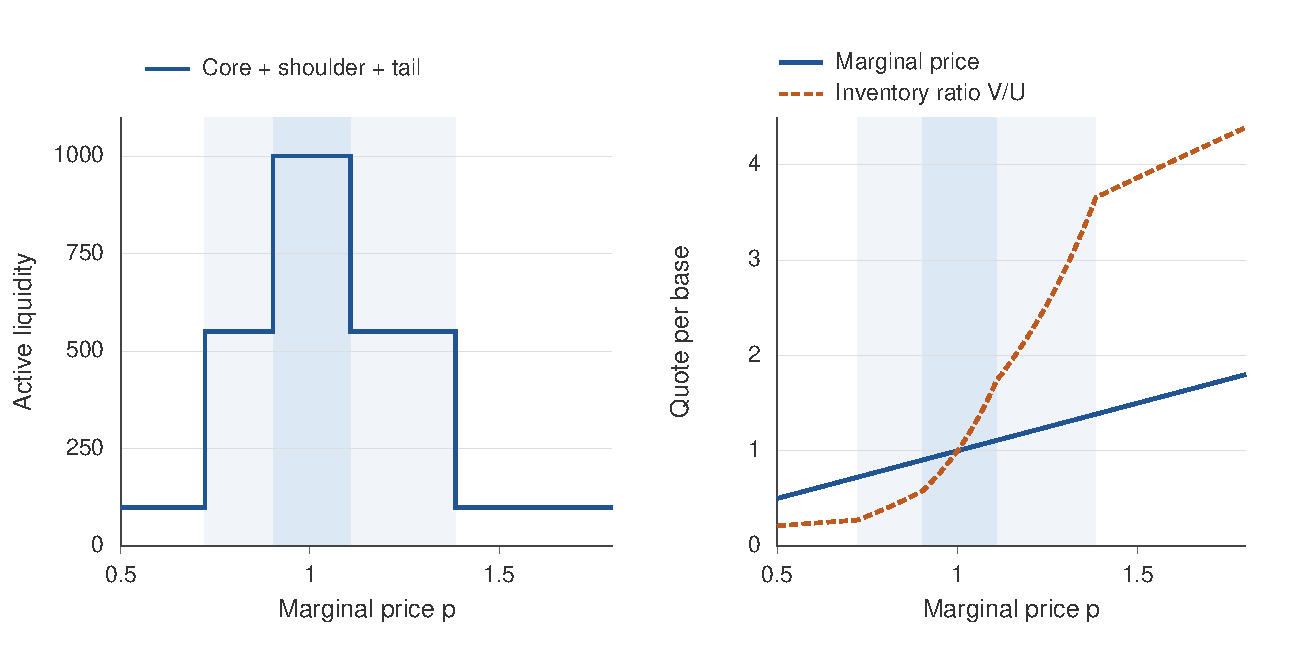
\includegraphics[width=0.96\linewidth]{simulations/figures/concentrated_curve.pdf}
\caption{An illustrative fixed nested geometry. Marginal price and inventory ratio remain continuous across the boundaries, while active liquidity changes by region. The dark core and light shoulder describe the same two ranges in both panels. The example is specified in the companion data.}
\label{fig:curve}
\end{figure}

\subsection{Center movement and fees}

The concentration center is persistent state. An eligible operation can commit a previously deferred controller target before preparing its quote. The new trade observation may schedule a later target; it does not first move the center using its own endpoint and then reprice itself against that center. Thresholds, an adjustment step, an interval, and economic admission checks constrain center movement.

The swap fee combines a base charge, an outward-divergence surcharge, and a volatility surcharge. The active path evaluates divergence over a gross trade path and limits the charge with component and aggregate budgets. It does not run the historical implicit fee solver. Volatility pricing uses decayed prior state, and a successful trade updates the signal used by later operations.

Fees can be collected on input, on base only, or on quote only. If the fee asset is input, the budget is measured on actual reserve credit after the input token transfer fee. If the fee asset is output, it is measured on gross curve output. In either case total Dusk swap fees are bounded by half of that fee basis, rounded down. Token-program transfer fees are additional; the bound is not a universal limit on the user's total loss from fees and price impact.

\subsection{Claimable yield and compounding}

A configured portion of eligible LP base fees and distributed dynamic surcharges can compound into principal. The remaining claimable swap yield is held outside executable reserves and distributed through growth indexes. Realized borrow interest follows its own distribution path. Thus the earlier description of all yield as universally non-compounding no longer applies.

For an eligible balance $s$, an index increment $\Delta G_i$ produces a yield increment of the form $s\Delta G_i$, with fixed-point scaling and fractional remainder handling in the implementation. Eligibility must be measured at the correct transition boundary: changing hLP ownership before allocating a fee could assign the trade's yield to a different set of shares.

Retained dynamic surcharge has another purpose. It enters $Z_i$ in equation~\eqref{eq:custody} and remains unavailable for swaps or harvest until an admitted recenter deploys it. It is not interchangeable with claimable yield, base-fee compounding, or unpaid interest. The controller's ability to move liquidity is therefore constrained by a specific funding source.

\ifexpanded
\subsection{Launch controls and recipient authority}

The fee profile includes an optional launch schedule. Its time decay can be linear or use a sixteen-step exponential schedule; an optional price-progress schedule also has a bounded duration. A directional size premium prices an individual qualifying buy. It is stateless across transactions, so splitting an order across transactions can reduce the premium. While the directional limiter is active, the program rejects multiple same-market swap-like top-level actions in one transaction. These rules do not imply a universal per-wallet trading quota or resistance to all forms of order splitting.

Yield ownership, destination, and execution authority are distinct. The yield-account owner can set the recipient and an optional harvest authority independently. The owner, recipient, or configured harvest authority may invoke harvest, but payout goes to the recipient's canonical associated token account for the mint and token program. The additional authority authorizes execution of harvest; it does not give the signer arbitrary payout routing. An owner that is a program-derived address can act through its program's signed invocation.

Compounding changes a reserve claim, whereas harvest settles a published liability. The integrated fee transition allocates value to the pre-swap eligible yLP ownership, converts each hLP's allocation into its target equity, and reconstructs the matching funding position. This is why simply adding the entire fee to one raw reserve after a trade is not a complete description of the current fee path.
\fi

\section{Leveraged Liquidity}
\label{sec:hlp}

The base hLP vault holds a funded yLP position whose net exposure targets base; quote hLP is symmetric. Let $E_b,E_q$ be their target-asset equities after accounting for the funding and yield effects included in the transition. In the continuous model, a canonical endpoint is
\begin{align}
X_b&=U+E_b+E_q\frac UV,&
D_b^{h,*}&=E_q\frac UV,\\
X_q&=V+E_q+E_b\frac VU,&
D_q^{h,*}&=E_b\frac VU.
\label{eq:endpoint}
\end{align}
The opposite-asset yLP claim and the target funding obligation match. For ordinary share supply $S_o$, vault-owned shares are reconstructed as
\begin{equation}
s_b=\left\lfloor\frac{S_oE_b}{U}\right\rfloor,\qquad
s_q=\left\lfloor\frac{S_oE_q}{V}\right\rfloor,\qquad
S=S_o+s_b+s_q.
\label{eq:ownership}
\end{equation}
These formulas describe aggregate vault state and require no scan over hLP holders.

The trader first receives a quote on $(U,V)$. The program then reconstructs the two vaults at the quoted endpoint and verifies the associated debt, cash, interest, and reserve changes. Synthetic hLP inventory is not an extra free tranche of trader depth. The earlier fixed-point pre-rebalance, bisection, and tracking-loss-threshold description is not the active integrated mechanism.

For base hLP, its gross LP value at marginal price $p$ is $E_bp+E_bV/U$, and debt value is $E_bV/U$. Relative to target equity value $E_bp$, gross leverage is
\begin{equation}
\mathcal L_b=1+\frac{V}{Up},\qquad
\mathcal L_q=1+\frac{Up}{V}.
\label{eq:leverage}
\end{equation}
Both equal two at a balanced constant-product point. With concentrated liquidity away from the center, inventory weights differ and a universal fixed-$2\times$ claim would be incorrect.

\subsection{Funding and settlement constraints}

An hLP deposit is admitted only if projected indexed funding debt fits the current borrowed-asset cash headroom. This is a deposit check, not a global theorem that funding debt remains below cash after every swap or after passive interest accrual. Integrated transitions also require cash to cover output and funding-interest settlement. A cash-constrained transition can reject; the paper makes no promise that it will continue by carrying an unfinished rebalance.

The implementation binds a prepared hLP transition to its expected pre-state. After applying the cash and funding effects, it checks the reconstructed executable endpoint within a fixed tolerance of three raw token atoms per side and asserts the stored reserve identity. Token normalization, indexed debt conversion, and share rounding remain part of that check. The zero residual-exposure field is an accounting result of reconstruction, not a guarantee against economic loss.

\subsection{Funding recovery and terminal closeout}

Let $D$ be actual indexed funding debt, $A$ the canonical opposite claim, and $Y$ revenue already available for netting. The recovery gap is
\begin{equation}
g=\pos{D-Y-A}.
\end{equation}
For positive $A$, recovery ignores gaps below 25 basis points of $A$. Above that threshold the discount is
\begin{equation}
d=\min\left(0.05,\frac{0.8g}{A}\right).
\label{eq:discount}
\end{equation}
It reaches its maximum at $g=A/16$. A spot swap supplying the borrowed asset can match $m=\min(g,\text{input})$. If that matched amount converts to a fair target amount $v$, the extra target output is
\begin{equation}
\beta=\min\left(E_t,\left\lfloor\frac{vd}{1-d}\right\rfloor\right).
\label{eq:bonus}
\end{equation}
The full trade still pays ordinary fees and follows the ordinary curve. The bonus consumes the selected hLP's equity. Critical stress is tested on actual debt before revenue netting, at $D/A\ge9/8$. The dedicated rescue path requires a positive critical recovery tranche and can run in reduce-only mode; it still requires the caller's swap input.

Terminal hLP closeout is narrower than arbitrary debt forgiveness. The implemented path accepts insolvency attributable to unpaid funding interest, requires the shortfall not to exceed interest due, retires the vault's yLP exposure, applies bounded insurance senior to residual interest socialization, and preserves previously published yield claims. A principal shortfall violates its invariant and rejects. A bounded caller bounty is funded from recovered interest. This is separate from ordinary borrower liquidation and from a routine hLP withdrawal.

\ifexpanded
\subsection{Leveraged liquidity and Yield Basis}

The constant-product LP convexity argument explains why two-times leverage is a useful reference point \cite{egorov-yieldbasis-whitepaper}. It does not prove that every concentrated LP portfolio has that leverage, or that funding and trading losses cancel. Yield Basis maintains leverage around externally held Curve LP collateral and crvUSD debt \cite{yieldbasis-technical}. Dusk instead matches opposite-asset claims and debt inside a pair-local endpoint reconstruction. Neither architectural description establishes a ranking of returns, costs, or resilience.

Dusk's target-asset equity can change through funding interest, fee allocation, recovery incentives, settlement, and market losses. A neutral opposite-asset claim at an admitted endpoint removes one accounting mismatch. It does not make target equity constant across every operation. In particular, equation~\eqref{eq:bonus} makes the cost of attracting recovery flow explicit: the trader's additional output is a reduction in hLP equity.
\fi

\section{Credit, Rates, and Liquidation}

\subsection{Borrow admission}

Public credit uses a shadow constant-product risk curve derived from the full-range tail, conservative depth, and internal price references. In a collateral-to-debt orientation, write
\begin{equation}
\widehat p=\min(p_{\rm symEMA},p_{\rm dirEMA}),\qquad
L_{\rm hist}=\min(L_{\rm observed},L_{\rm EMA}).
\end{equation}
When one historical depth observation is zero, the nonzero observation is used. Write $L_{\rm total}=L_0+L_{\rm concentrated}$ for current prepared center depth. The shadow liquidity scales only the tail:
\begin{equation}
\widehat L_0=L_0\frac{\min(L_{\rm hist},L_{\rm total})}{L_{\rm total}},
\end{equation}
with $\widehat L_0=L_0$ when historical depth is unavailable. The conceptual risk reserves are $\widehat x=\widehat L_0/\sqrt{\widehat p}$ and $\widehat y=\widehat L_0\sqrt{\widehat p}$. Impact-aware value is
\begin{equation}
W(c)=\frac{c\widehat y}{\widehat x+c}.
\label{eq:risk}
\end{equation}
The full concentrated execution curve is not simply substituted into borrow admission. The public-borrow book also maintains debt-capped aggregate underwriting contributions; those aggregate contributions do not lock other accounts' idle collateral.

A successful public borrow recomputes and stores the position's liquidation collateral factor, subject to the borrower's minimum acceptable factor. Borrow capacity uses a five-percent buffer below that factor. On collateral withdrawal the check uses the greater of the stored and newly computed factor, then tests the post-withdrawal buffered capacity. Full repayment clears the factor. Each debt side is secured by that position's opposite-asset collateral.

Public cash borrowing additionally consumes a leaky 24-hour budget derived from conservative depth. The default limit is 20 percent and the configurable ceiling is 30 percent of the relevant depth measure. Only new gross public borrow consumes this budget; repayment does not refill it immediately. hLP funding and isolated leverage do not consume this particular public-borrow bucket, although both face their own checks and enter utilization.

\subsection{Adaptive interest}

For each asset, utilization includes all indexed debt without double counting:
\begin{equation}
u_i=\frac{D_i^f+D_i^\ell+D_i^h}{D_i^f+D_i^\ell+D_i^h+C_i}.
\end{equation}
The default target is $u^*=0.70$, with normalized error
\begin{equation}
e(u)=\begin{cases}(u-u^*)/u^*,&u\le u^*,\\(u-u^*)/(1-u^*),&u>u^*.
\end{cases}
\end{equation}
For curve steepness $\kappa$, the instantaneous APR is $r=r_Tc(e)$, where
\begin{equation}
c(e)=\begin{cases}1+(\kappa-1)e,&e\ge0,\\1+(1-1/\kappa)e,&e<0.
\end{cases}
\end{equation}
The default $\kappa=4$ gives multipliers from $1/4$ to $4$. Dusk uses the adaptive-anchor idea associated with Morpho's AdaptiveCurveIRM \cite{morpho-irm-github}, with a bounded linear update
\begin{equation}
r_T'=\clip\left(r_T\left[1+\clip(se\tau,-0.5,0.5)\right],0.001,2\right),
\label{eq:irm}
\end{equation}
where $\tau$ is elapsed time in years, capped at one year per update, and default speed is $s=20$. The anchor starts at four percent APR. Its 0.1--200 percent bounds apply to the anchor, not the final borrower APR after multiplication.

The program accrues the borrow index at the rate computed from the pre-update state, then updates the anchor. Elapsed time is inferred from slots at 400 milliseconds per slot. Debt and index arithmetic round in integer fixed point, so continuous-time formulas or a particular update cadence must not be presented as bit-for-bit execution under arbitrary activity.

\subsection{Liquidation and isolated leverage}

Public liquidation eligibility uses debt versus the position's stored liquidation factor and a linear mark at the symmetric price EMA. Auction pricing is a different calculation: the floor is the average full-position concentrated unwind value using the symmetric reference price and pessimistic depth. The auction starts at a five-percent premium to that floor and decays over five minutes. External fillers repay in the debt asset and receive collateral under the auction terms.

After expiry, the backstop can unwind through the live curve, pay a 0.5-percent bounty on consumed collateral, apply capped insurance, and socialize residual loss in the market. Surplus debt-asset proceeds return to the borrower. Insurance has hard concentration ceilings of 20 percent per event and 50 percent per slot-based day window; governance can impose lower limits. These insurance limits are not a guarantee that LP losses cannot exceed a fixed percentage.

Isolated spot-margin leverage has its own collateral and debt shares. In an idealized opening, margin $m$ and multiplier $\mathcal L$ imply borrowing $m(\mathcal L-1)$ and swapping the resulting notional through the market. Actual entry pays fees, impact, and applicable transfer costs. Initial and maintenance health use position closeout value and unwind constraints, rather than public-borrow aggregate contributions. Increases, decreases, closeout, and liquidation reuse the concentrated swap and cash settlement machinery. A conditional order or liquidation trigger establishes permission to attempt execution, not a guaranteed fill.

\ifexpanded
\subsection{Conditional execution and market controls}

The leverage-delegate program supports delegated take-profit and stop-loss closeouts, escrowed leverage entries with limits and expiry, and hLP stop orders. hLP stop-loss uses principal NAV per share; its stop-rate condition uses a fixed twelve-hour EMA of funding APR. An hLP order preserves the original owner's yield destination while shares are escrowed. Execution deducts a five-percent output bounty, rounded up, before applying the owner's payout bound; token transfer fees can still affect final receipt. Residual published yield can be settled after the order leaves escrow.

Parameter governance exposes seven families: fees, concentration, interest, EMA half-lives, public daily borrow limits, the center controller, and insurance draw caps. Proposal timing and execution conditions are part of the implementation. Market start state, liquidity gates, and reduce-only controls can constrain individual instructions. Their presence describes available control mechanisms; it does not establish a production deployment or a release policy.
\fi

\section{Numerical Illustrations and Limitations}

The companion generator replaces the old synthetic-depth and discrete pre-rebalance experiments with three illustrations of the current mechanism. It produces the tables and vector figures used by the two drafts. Inputs are disclosed in the generated metadata. The curve illustration holds a chosen geometry fixed; the rate illustration updates once per day at fixed utilization; recovery examples use the integer discount and bonus rules. None runs the complete Solana program.

\begin{center}
\begin{tabular}{@{}lrr@{}}
\toprule
Fixed utilization & Day-30 anchor APR & Day-30 borrower APR \\
\midrule
0\% & 0.7376\% & 0.1844\% \\
70\% & 4.0000\% & 4.0000\% \\
100\% & 19.8196\% & 79.2786\% \\
\bottomrule
\end{tabular}
\end{center}


The rate rows use $u^*=70\%$, $\kappa=4$, $s=20$, and an initial four-percent anchor. The concentrated example uses a positive tail and equal core/shoulder layer liquidities to display the five regions. It is an illustrative geometry, not a recommended deployment configuration. Recovery figures distinguish the 25-basis-point activation threshold, maximum discount at a gap of $1/16$, and the separate critical test on actual debt.



Several limitations follow from the model. Cash exhaustion can prevent an otherwise valid quote or withdrawal from settling. Internal price filters can lag or be manipulated, and a positive full-range tail does not guarantee useful size at every price. Funding growth can erode hLP equity even when opposite claims are reconstructed correctly. Auction participation, rescue flow, and permissionless terminal calls remain liveness assumptions. Insurance and explicit loss accounting determine how losses are allocated; they do not supply unlimited capital.

The implementation also has finite arithmetic precision, state-dependent fees, and operation ordering that a continuous derivation cannot certify. The most useful next empirical work is exact-program replay across cash stress, boundary crossings, funding recovery, and liquidation, with fee and funding costs included. Historical prototype benchmarks should not be used as measurements of this source snapshot. This revision reports no throughput, return, or comparative performance result.

\section*{Reproducibility}

Both papers share the same mechanism source so that corrections to equations and parameters remain consistent. \src{paper/simulations/generate.py} generates the numerical data, summary table, and vector figures. \src{paper/SOURCES.md} maps claims to implementation paths and describes the verification scope. The expanded appendices provide derivations, worked examples, and a transition-level review map. Code remains the authority for rounding, account validation, instruction ordering, and rejection conditions.

\ifexpanded
\begin{figure}[htbp]
\centering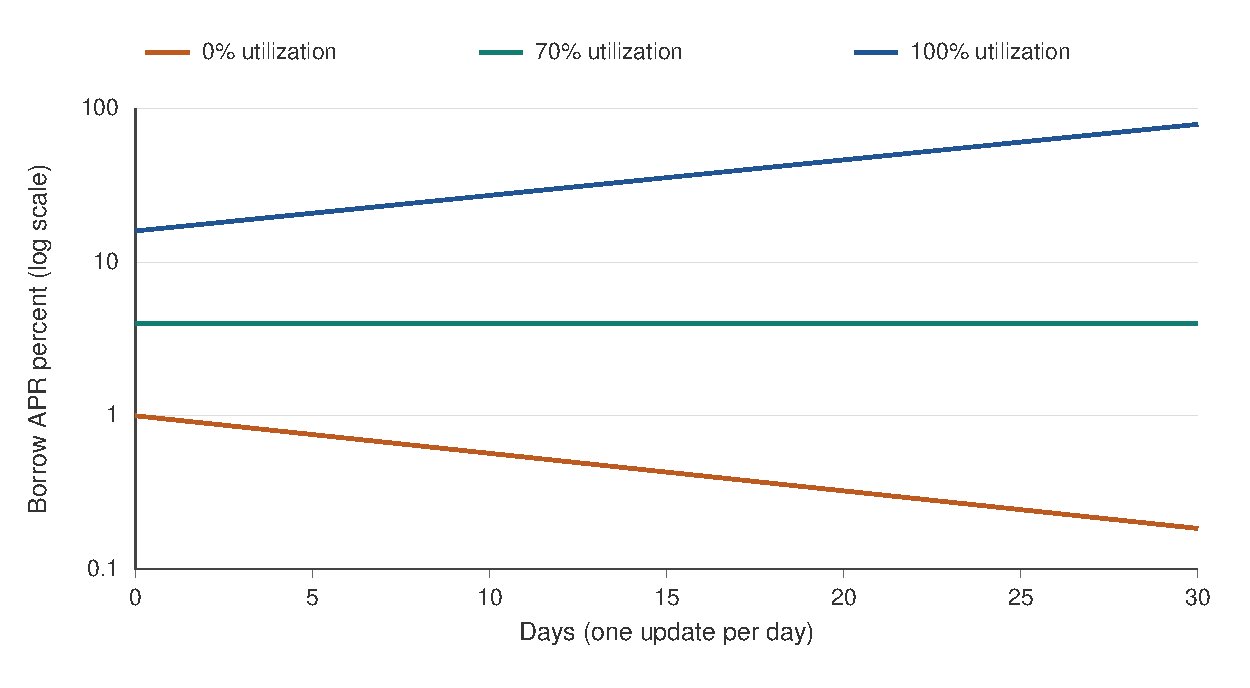
\includegraphics[width=0.88\linewidth]{simulations/figures/adaptive_irm.pdf}
\caption{Fixed-utilization rate paths with one anchor update per day and current default parameters. Values show the instantaneous APR after each update. This cadence is part of the experiment, not a claim of cadence-independent onchain accrual.}
\label{fig:irm}
\end{figure}
\begin{figure}[htbp]
\centering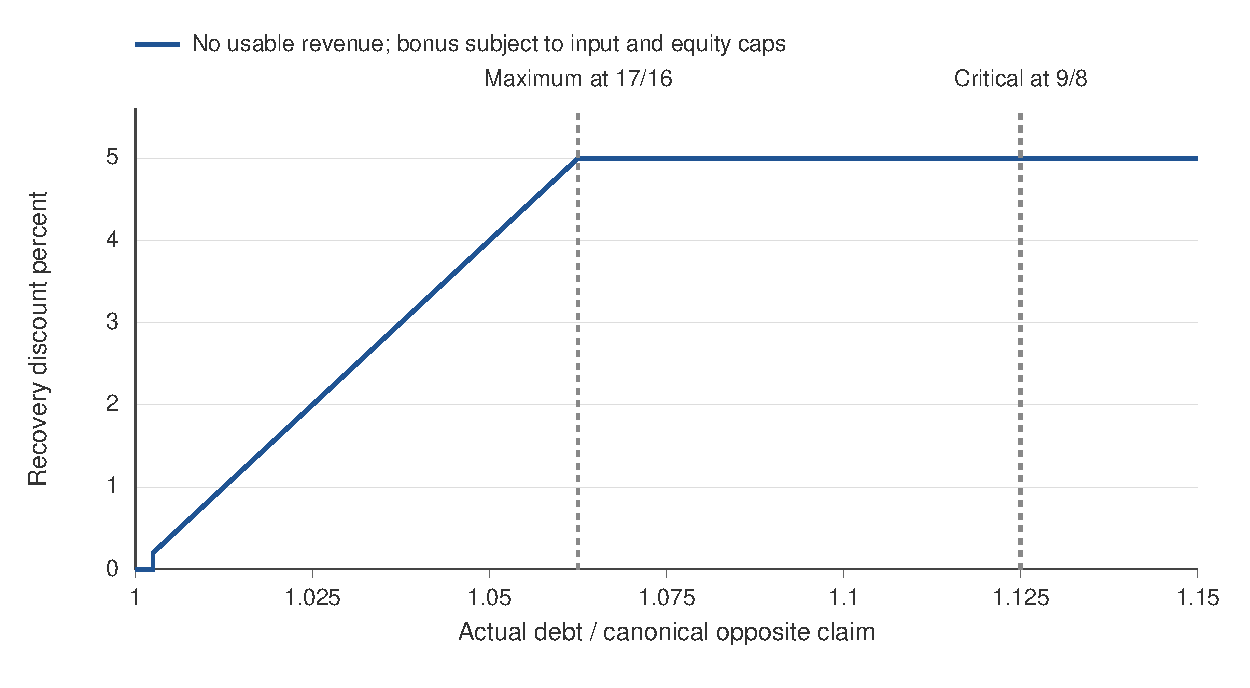
\includegraphics[width=0.88\linewidth]{simulations/figures/hlp_recovery.pdf}
\caption{Recovery discount with no usable revenue. Maximum discount occurs at debt/claim $17/16$; critical stress begins at $9/8$. The plotted fine-scale discontinuity at 25 basis points reflects the activation guard. Bonuses also depend on matching input, conversion ratio, integer rounding, and available equity.}
\label{fig:recovery}
\end{figure}
\fi
